

\begin{frame}{Le champ de croix}{Définition, caractéristiques, ...}
    \begin{columns}
        \begin{column}{0.6\textwidth}
            \centering
            \includegraphics[scale=0.18]{img/valence.pdf}\\\vspace{0.3cm}
        \end{column}
        \begin{column}{0.4\textwidth}
            \begin{onerablock}[hbox,drop fuzzy shadow,sharp corners]{\small Nombre de séparatrices (Valence)}
            \vspace{0.5cm}
            $
            \hspace{1.2cm}
            V(p)=4-4id(p)
            \hspace{1.2cm}
            $
            \vspace{0.5cm}
            \end{onerablock}
        \end{column}
    \end{columns}
    \begin{columns}
        \begin{column}{0.4\textwidth}
            \centering
            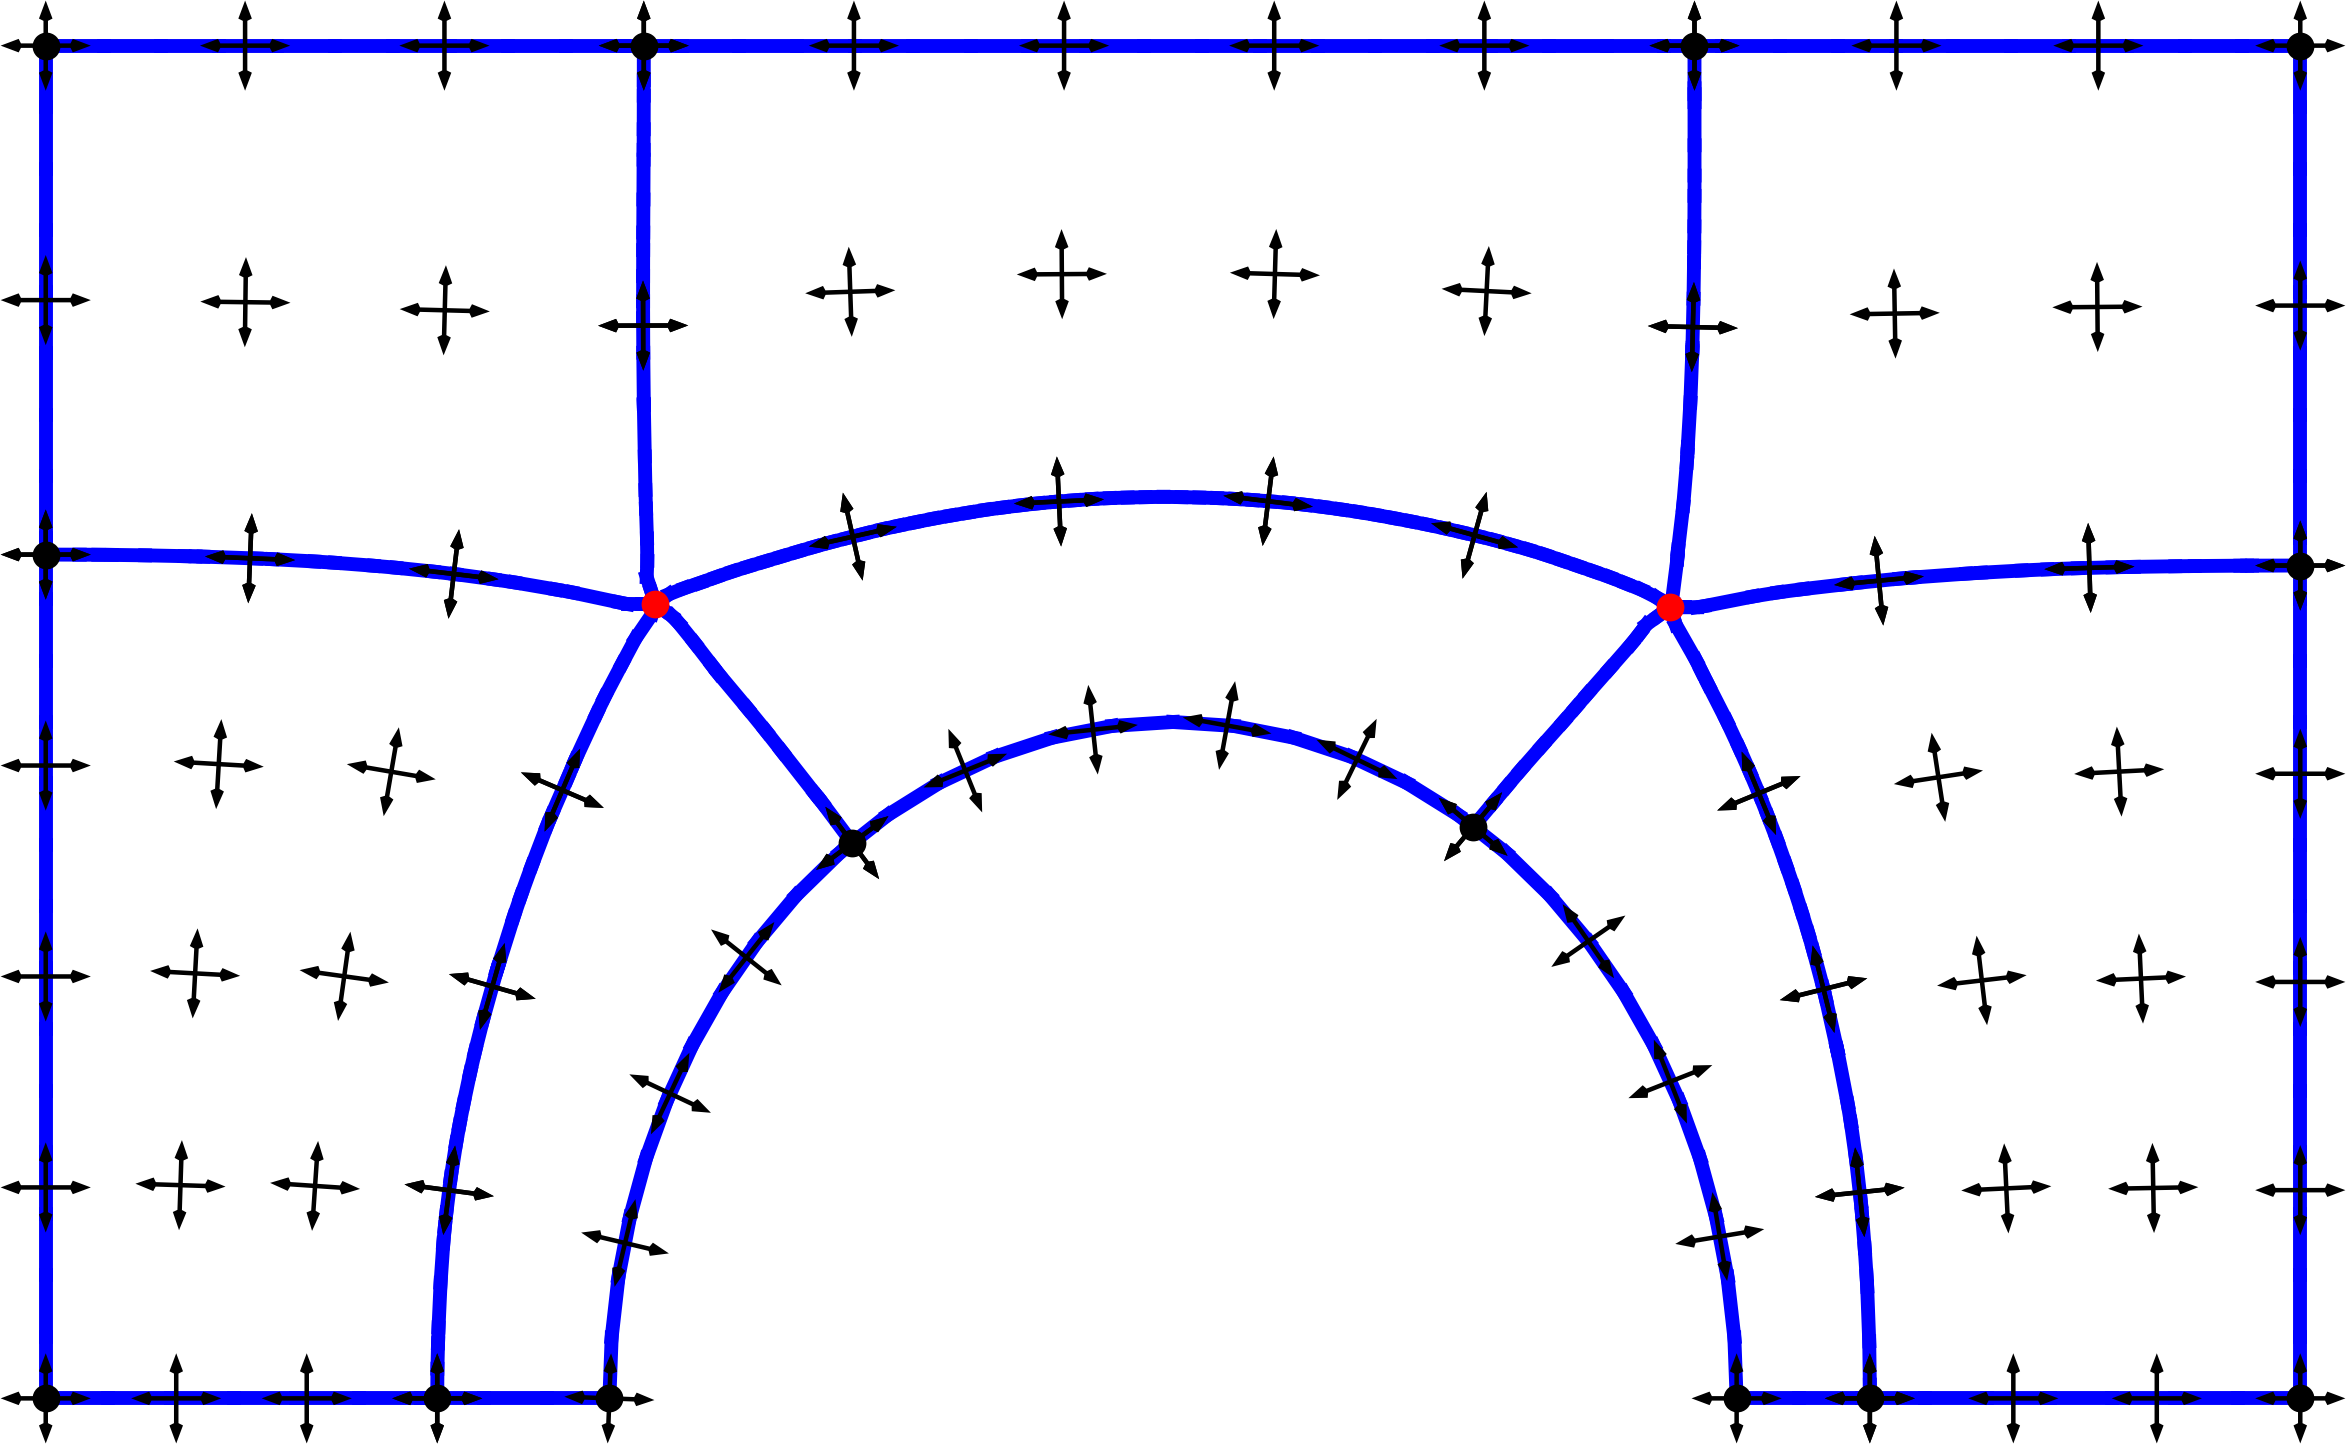
\includegraphics[scale=0.26]{img/frey_3.png}\\\vspace{0.15cm}
            \caption{\footnotesize Partitionnement}
        \end{column}
        \begin{column}{0.6\textwidth}
            Soit $\mathcal{R}$ l'une des régions, On a:
    $$\chi(\mathcal{R})=1=\sum_{i=1}^{n_c}id_u(c_i)=\sum_{i=1}^{n_c}\frac{1}{4}\Longrightarrow n_c=4$$
    Ce qui implique que $\mathcal{R}$ a 4 coins par rapport au champ de croix.
        \end{column}
    \end{columns}
\end{frame}

    \begin{frame}{Formalisation du processus de partitionnement}{Partitionnement à partir d'un champ de croix aligné}
    \begin{onerablock}[drop fuzzy shadow]{Théoreme 1}
    Si $\bar{u}$ est un champ de croix tangent au bord du domaine tel que $id_{\bar{u}}(p) = d/4,~\forall p\in\Omega, d\in\mathbb{Z},d\leq 1$  et qu'aucune de ses séparatrices ne converge en cycle limite alors ils partitionnent $\Omega$ en régions de 4 côtés.
    \end{onerablock}
    \vspace{0.4cm}
    \begin{onerablock}[drop fuzzy shadow]{Lemme}
    Une région est de 4 côtés par rapport au champ de croix si et seulement si il possède uniquement 4 points singuliers de bord d'index 1/4.
    \end{onerablock}
    \vspace{0.4cm}
    \end{frame}

    \begin{frame}{Le champ de croix}{Définition, caractéristiques, ...}
    \begin{columns}
        \begin{column}{0.6\textwidth}
            \centering
            \includegraphics[scale=0.18]{img/valence.pdf}\\\vspace{0.3cm}
        \end{column}
        \begin{column}{0.4\textwidth}
            \begin{onerablock}[hbox,drop fuzzy shadow,sharp corners]{\small Nombre de séparatrices (Valence)}
            \vspace{0.5cm}
            $
            \hspace{1.2cm}
            V(p)=4-4id(p)
            \hspace{1.2cm}
            $
            \vspace{0.5cm}
            \end{onerablock}
        \end{column}
    \end{columns}
    \begin{columns}
        \begin{column}{0.4\textwidth}
            \centering
            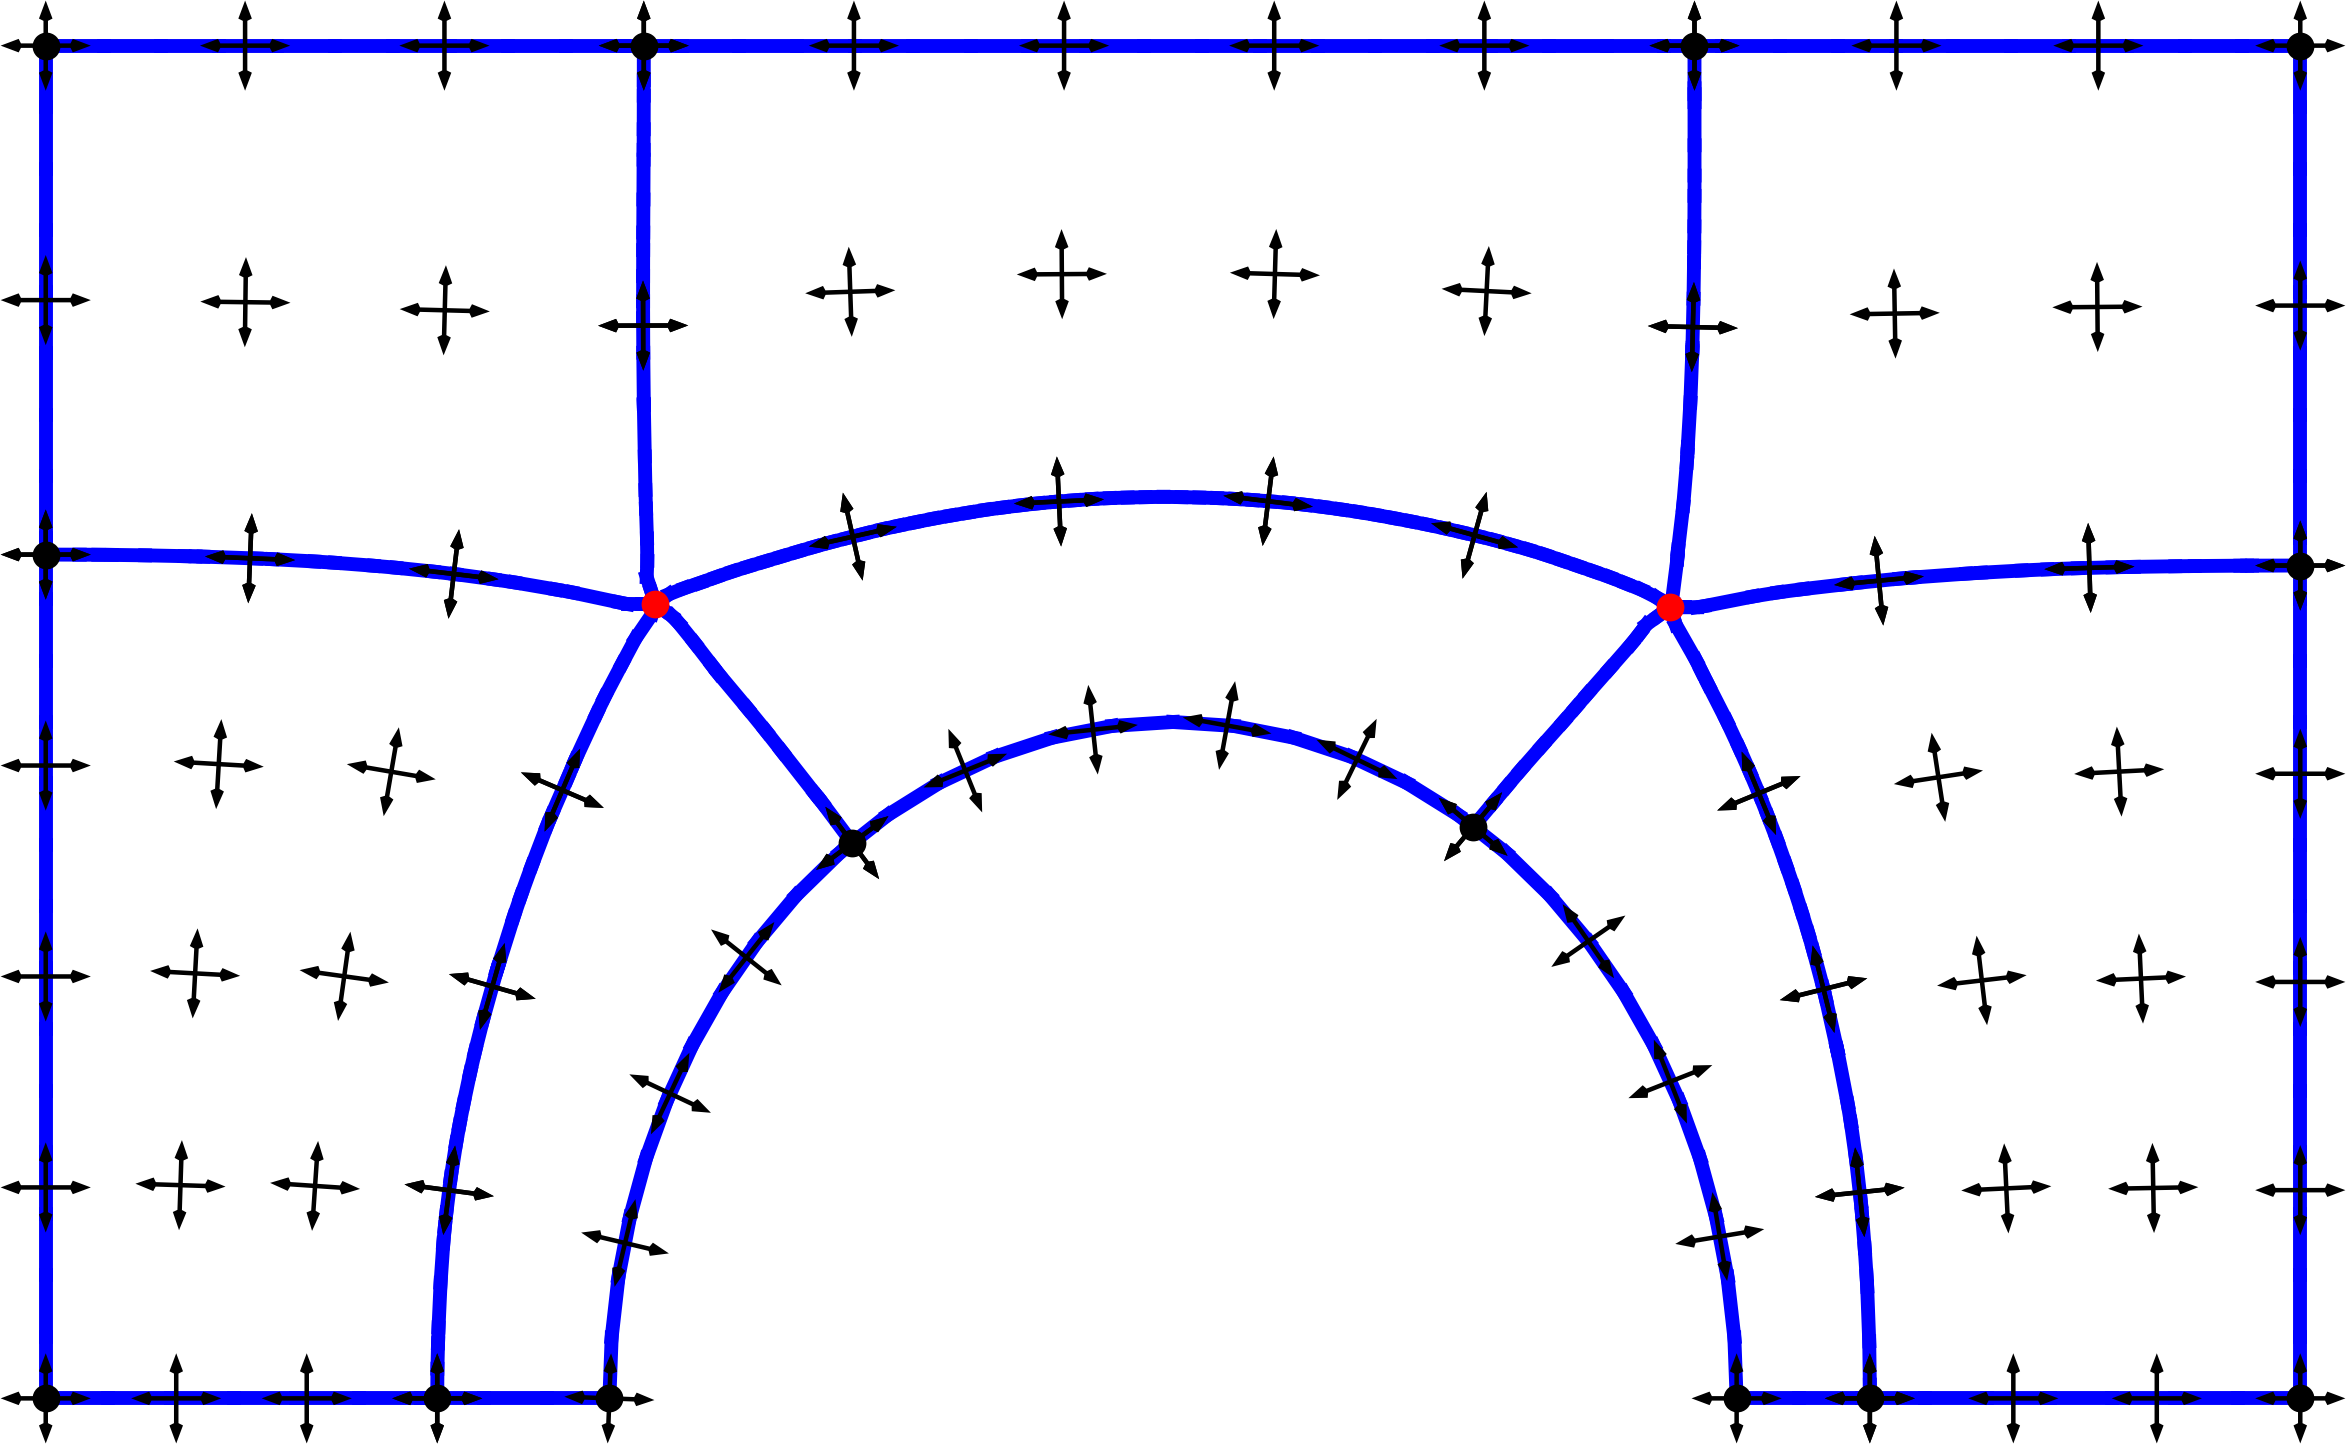
\includegraphics[scale=0.26]{img/frey_3.png}\\\vspace{0.15cm}
            \caption{\footnotesize Partitionnement}
        \end{column}
        \begin{column}{0.6\textwidth}
            Soit $\mathcal{R}$ l'une des régions, On a:
    $$\chi(\mathcal{R})=1=\sum_{i=1}^{n_c}id_u(c_i)=\sum_{i=1}^{n_c}\frac{1}{4}\Longrightarrow n_c=4$$
    Ce qui implique que $\mathcal{R}$ a 4 coins par rapport au champ de croix.
        \end{column}
    \end{columns}
\end{frame}

\begin{frame}{Point de vue}
    \vspace{-0.35cm}
    \begin{columns}
        \begin{column}{0.33\textwidth}
            \centering
            \begin{figure}
                \centering
                \includegraphics[scale=0.12]{img/point_of_view_1.png}\\\vspace{0.1cm}
                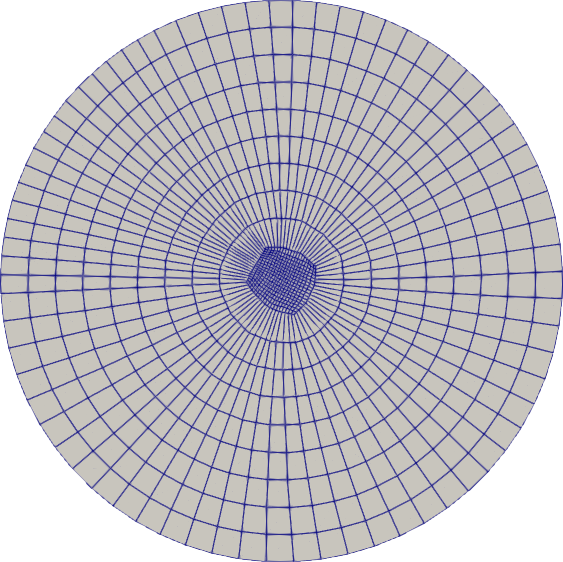
\includegraphics[scale=0.12]{img/new_cercle.png}
                \caption{Propagation de la normal}
            \end{figure}
        \end{column}
        \begin{column}{0.33\textwidth}
            \centering
            \begin{figure}
                \centering\includegraphics[scale=0.28]{img/point_of_view_3.pdf}\\\vspace{0.2cm}
            \includegraphics[scale=0.25]{img/point_of_view_4.pdf}
                \caption{Mode propre}
            \end{figure}

        \end{column}
        \begin{column}{0.33\textwidth}
            \centering
            \begin{figure}
                \centering
            \includegraphics[scale=0.32]{img/point_of_view_5.pdf}\\\vspace{0.1cm
            }
            \includegraphics[scale=0.32]{img/point_of_view_6.pdf}
                \caption{Formule analytique}
            \end{figure}
        \end{column}
    \end{columns}
\end{frame}

\begin{frame}{Notre approche}
\pause[1]
    \begin{columns}
        \begin{column}{0.33\textwidth}
        \centering
        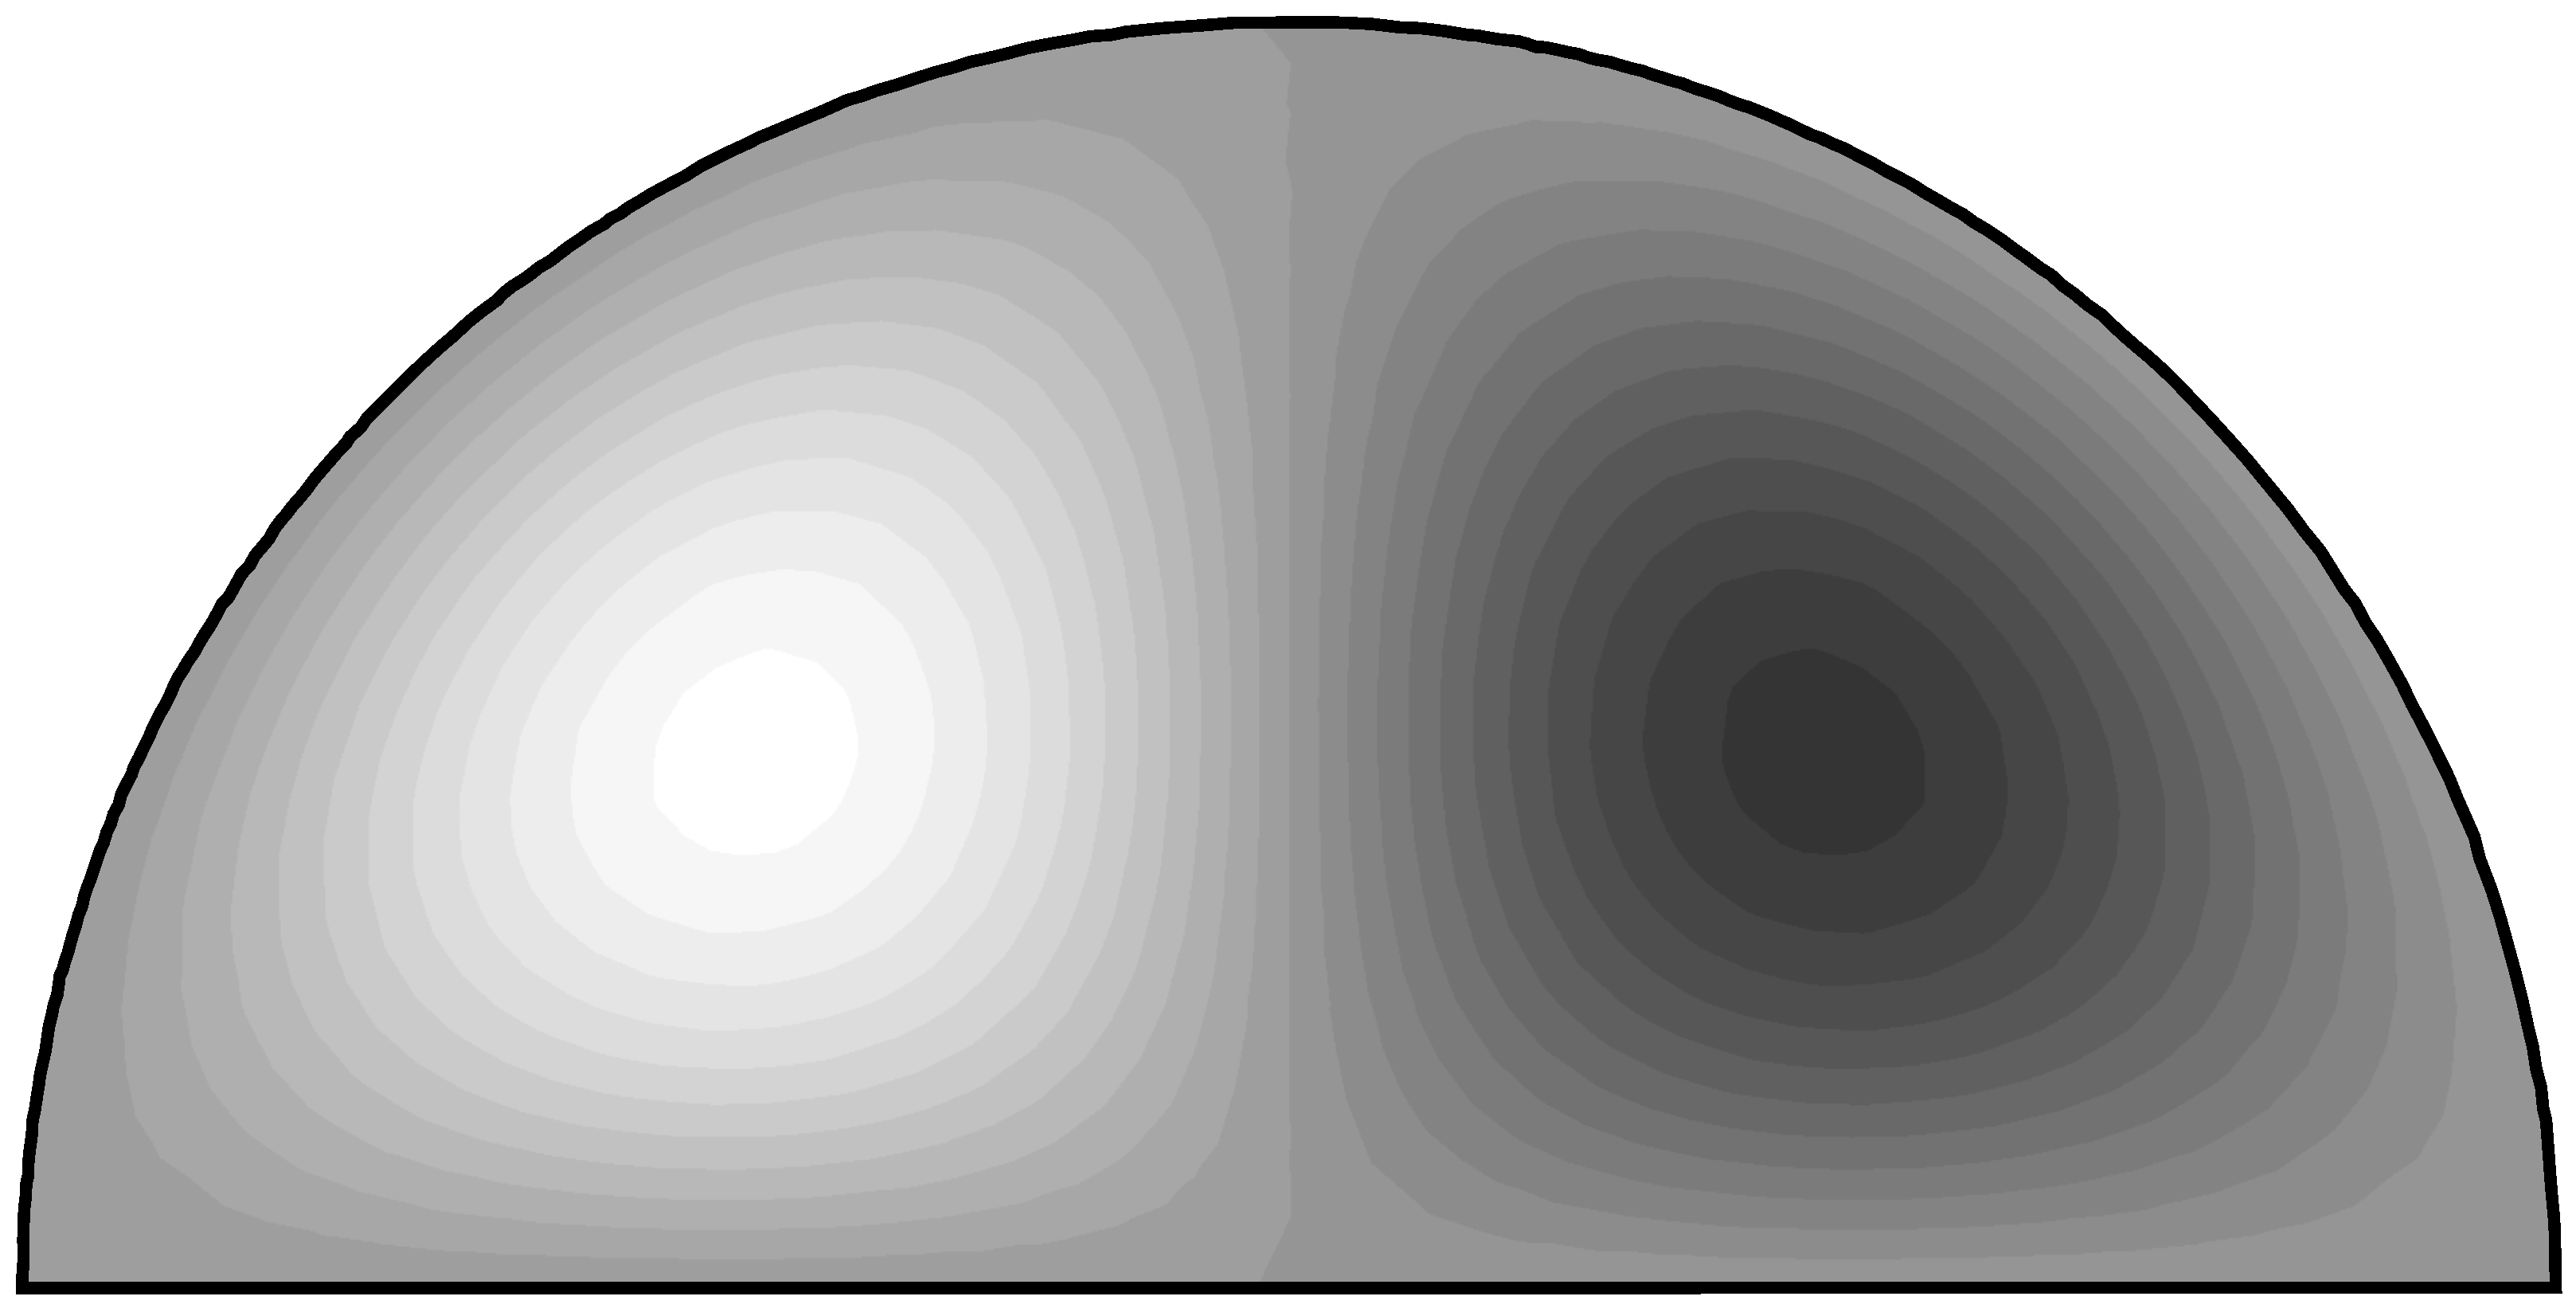
\includegraphics[scale=0.08]{images/demiDiscValProp.eps} \hspace{0.2cm}
        \caption{\footnotesize Eigenmode on half-disk}
        \end{column}
        \begin{column}{0.33\textwidth}
        \centering
        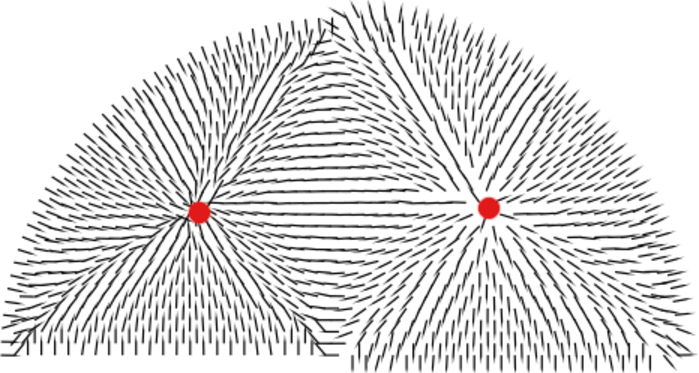
\includegraphics[scale=0.36]{images/val_prop_7.pdf} \hspace{0.2cm}
        \caption{\footnotesize Gradient}
        \end{column}
        \begin{column}{0.33\textwidth}
        \centering
        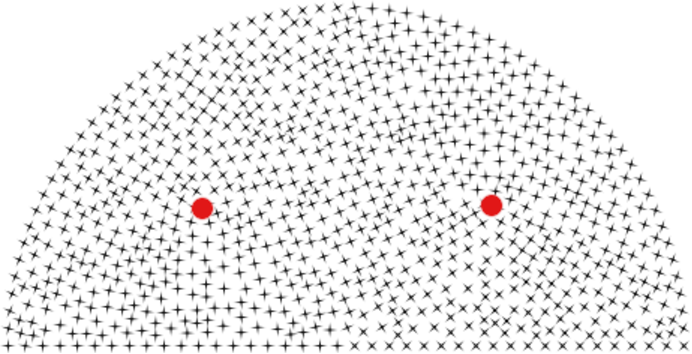
\includegraphics[scale=0.36]{images/demiDiscValPropSheet_2.pdf} \hspace{0.2cm}
        \caption{\footnotesize Champ de croix}
        \end{column}
    \end{columns}
\pause[2]
    \begin{columns}
        \begin{column}{0.5\textwidth}
        %\only<1>{
            \underline{\bf \'Etape}\\
            \begin{enumerate}
                \item \sout{Propagation de la normale} (Traitement d'un champ de croix "input")\\
                \item Détection des points singuliers
                \item Partitionnement du domaine
                \item "Mesh quad" de chaque partition
            \end{enumerate}
        %}
        \end{column}
        \begin{column}{0.5\textwidth}
             \centering
            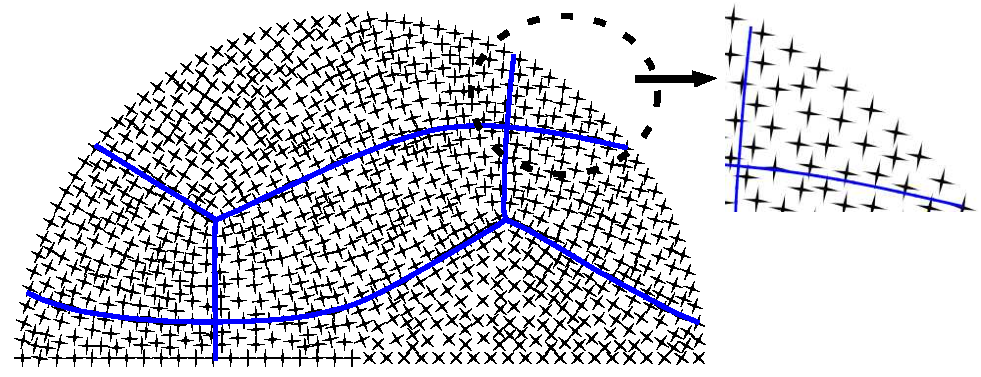
\includegraphics[scale=0.45]{img/gagaga.pdf}
            \vspace{0.2cm}
            \caption{\footnotesize Certaines partitions ne sont pas de 4 côtés}
            \vspace{0.5cm}
        \end{column}
    \end{columns}
\end{frame}





\begin{frame}{Champ d'alignement sur $\partial\Omega$}
    \vspace{-0.2cm}
    \begin{columns}
    \begin{column}{0.7\textwidth}
    Soit $u$ un champ de croix "input".\\\vspace{0.12cm}
    \textbf{Idée}: Trouver $\phi$ au moins $\mathcal{C}^0(\mathring{\Omega})$ tel que {\color{red}$v=R(\phi)u$} soit tangent à $\partial\Omega$ {\color{onera_gray}(Conservation des propriétés de $u$)}.\\\vspace{0.12cm}
    La normale est définie par $\theta_N=\Tilde{\theta_N}+\delta\theta_N$\\\vspace{0.14cm}
    \small
    {\bf Correction de la différence angulaire entre $u$ et $N$:}
    \vspace{-0.1cm}
    \begin{equation*}
    \left\{
    \begin{array}{lcl}
    \triangle\phi &=& 0 \mbox{ dans }\Omega,\\[0.1cm]
    \phi(\gamma(t)) &=& \Tilde{\theta_N}(\gamma(t))-\theta_u(\gamma(t)) + \color{red}\displaystyle\sum_{i=1}^{n_b}\delta\theta_N(c_i)\mathbb{1}_{\gamma([0, t])}(c_i)\color{black},~~\forall t\in[0, 1].
    \end{array}
    \right.
    \label{eq:phi_computation}
    \end{equation*}
    \vspace{-0.5cm}
    \footnotesize
    \begin{table}[!h]
    \centering
    \begin{tabular}{|c|c|c|c|c|}
    \hline
    \multirow{2}{*}{$\widehat{c_i}$} & \multirow{2}{*}{$\pi/2$} & \multirow{2}{*}{$\pi$} & \multirow{2}{*}{$3\pi/2$} & \multirow{2}{*}{2\pi/10} \\
    &&&&\\
    \hline
    \multirow{2}{*}{$id(c_i)$} & \multirow{2}{*}{$1/4$}   & \multirow{2}{*}{$0$}   & \multirow{2}{*}{$-1/4$} & \multirow{2}{*}{?}   \\
    &&&&\\
    \hline
    \end{tabular}
    %\caption{\tiny Usual distribution $\delta\theta_N(c_i)$ vs $id(c_i)$}% \textbf{angle-index} }%\cite{macq2020ginzburglandau}.}
    \label{tabul}
    \end{table}
    \vspace{-0.1cm}
    \centering \scriptsize Distribution usuelle $\widehat{c_i}$ vs $id(c_i)$\\

    \end{column}
    \begin{column}{0.3\textwidth}
        \centering
        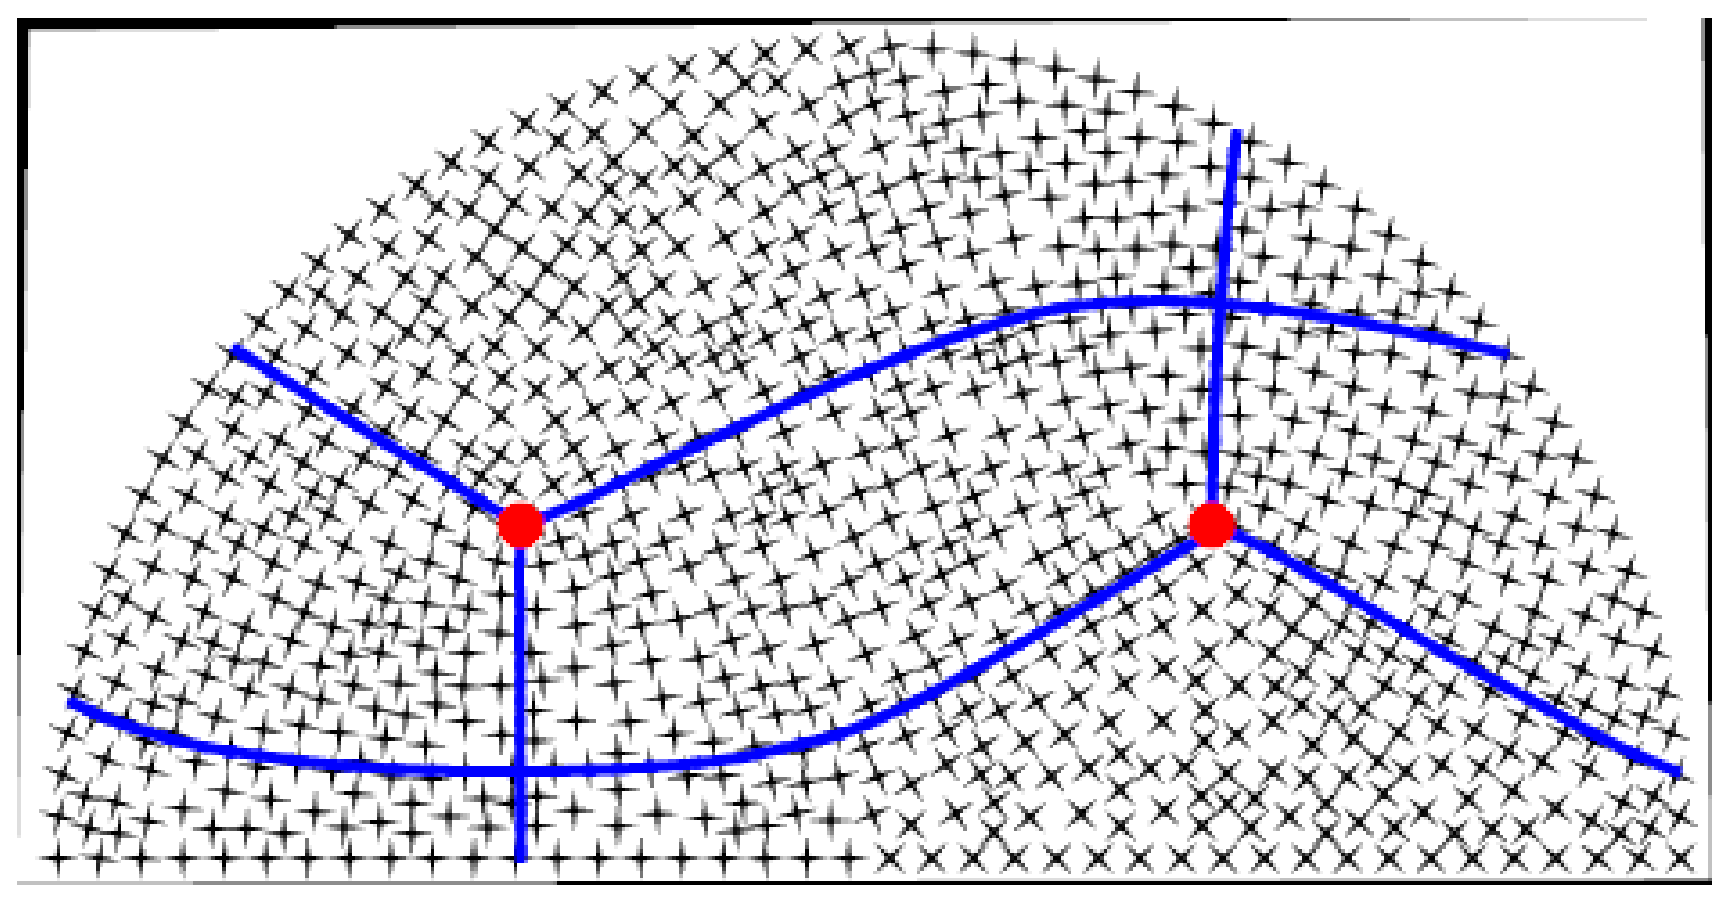
\includegraphics[scale=0.31]{demiDiscValPropNonAligne.eps}
        \caption{\footnotesize Champ de croix "input"}\\\vspace{0.5cm}
        \includegraphics[scale=0.22]{img/delta_theta_N.pdf}
        %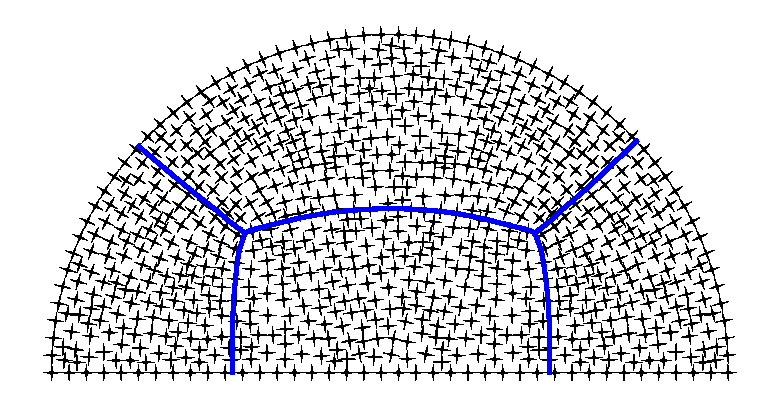
\includegraphics[scale=0.31]{demiDiscValPropAligne.eps}\\
        %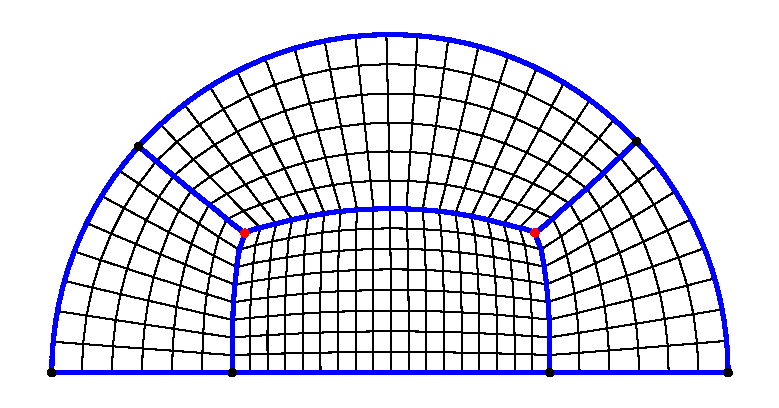
\includegraphics[scale=0.31]{mailDemiDisc.eps}\\\vspace{0.5cm}
    \end{column}
    \end{columns}
\end{frame}

\begin{frame}{Traitement des singularité de bord}{}
\vspace{-0.2cm}
\hspace{-0.35cm}{\bf \color{onera_gray} Prise en compte des conditions de bord, flag de matériau de bord, ...  }\\
\vspace{0.1cm}
\begin{columns}
\begin{column}{0.55\textwidth}
\small
soit $c\in\partial\Omega$ et $\gamma:[0,1]\rightarrow\Omega$ tel que $\gamma(0)=\gamma(1)=c$. Soit $I(c)$ l'index souhaité en $c$ i.e. $id_v(c)=I(c)$.
\vspace{-0.25cm}
    \begin{eqnarray*}
    id_v(c)&=&\frac{1}{2\pi}\int_\gamma d\theta_v\\
    &=&\frac{1}{2\pi}[\underbrace{\kappa_g(c)}_{\pi-\hat{c}}+\lim\limits_{s\rightarrow 0}\int_s^{1-s}d((\phi+\theta_u)\circ\gamma)]\\
    &=&\frac{1}{2\pi}[\pi-\hat{c}+\underbrace{\lim\limits_{s\rightarrow 0}\int_s^{1-s}d((\theta_N-\theta_u+\delta\theta_N+\theta_u)\circ\gamma)}_{\delta\theta_N(c)}]
    \end{eqnarray*}
    \vspace{-0.8cm}

\begin{onerablock}[hbox,drop fuzzy shadow,sharp corners]{\footnotesize Relation Angle-index}
\centering
$
\delta\theta_N(c) = 2\pi id_v(c)-\pi+\hat{c}
$
\end{onerablock}
\end{column}
\begin{column}{0.45\textwidth}
\centering
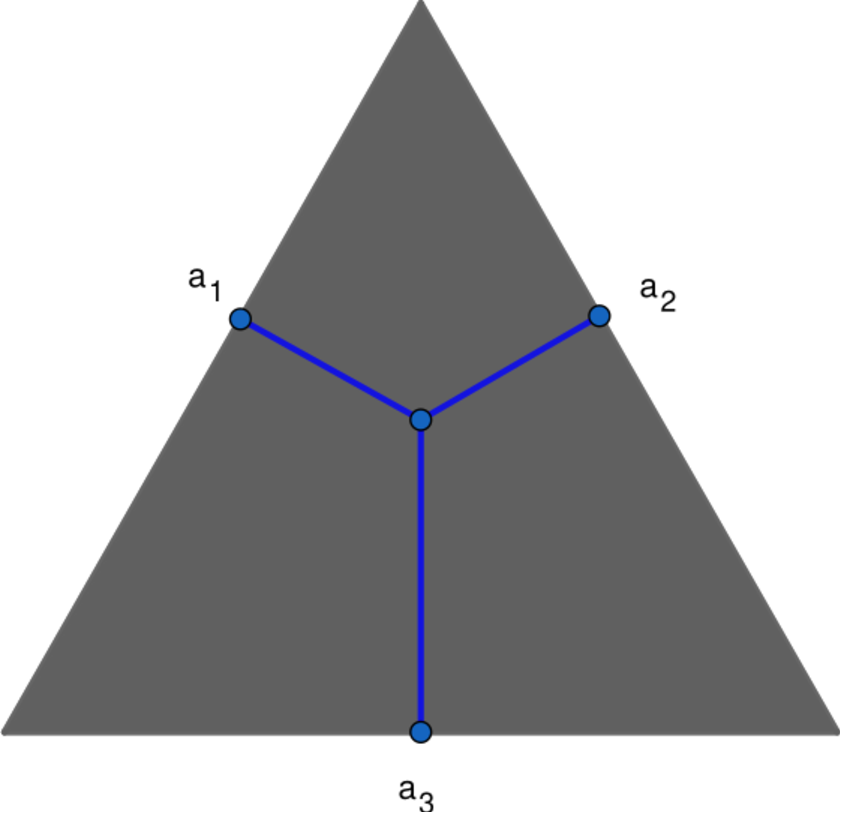
\includegraphics[scale=0.18]{img/geogebra-export.pdf}\\\vspace{0.2cm}
\includegraphics[scale=0.25]{img/bandit.pdf}
%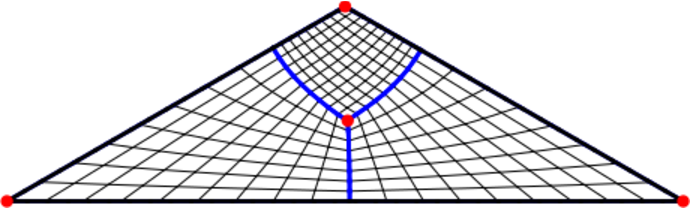
\includegraphics[scale=0.38]{img/mesh_quad_5.pdf}
%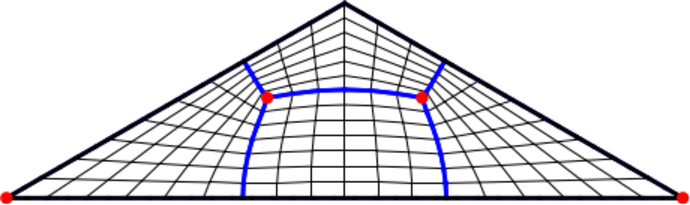
\includegraphics[scale=0.38]{img/mesh_quad_4.pdf}
\end{column}
\end{columns}
\end{frame}

\begin{frame}{Conservation des propriétés du champ de croix "input"}
\vspace{-0.2cm}
\small
À partir du théorème de Poincarré-Hopf,
\begin{equation*}
\sum_{s\in Int(\Omega)} id_v(s)+\sum_{c\in \partial\Omega} id_v(c) = \chi(\Omega),
\label{poincareformula_3}
\end{equation*}

on dégage une contrainte générale sur le champ de croix "input":
\begin{equation}
deg(u, \partial\Omega) =\sum_{s\in Int(\Omega)} id_u(s) = \sum_{s\in Int(\Omega)} id_v(s) = \chi(\Omega)-\sum_{c\in \partial \Omega} id_v(c).
\label{third_u_c}
\end{equation}
\begin{onerablock}[drop fuzzy shadow]{Théorème 2}
Soit $u$ un champ de croix tel que $\forall p\in\bar{\Omega}$, ${\bf id(p)<=1/4}$. \'Etant donné un ensemble $(c_i)_{i\in\{1,\dots,n_b\}}\subset\partial\Omega$ de points distincts tel que:
$
{\bf deg(u, \partial\Omega) = \chi(\Omega)-\sum_{i=1}^{n_b} id(c_i),}
$
il existe un champ de croix $v$ vérifiant le théorème 1.
\end{onerablock}
\vspace{0.1cm}
{\bf Remarque:}
La condition (\ref{third_u_c}) implique la périodicité de $\phi$.
\end{frame}


\begin{frame}{\fontsize{12}{12}\selectfont Quelques maillages résultant de différents choix du champ de croix "input"}
\vspace{-0.28cm}
\begin{columns}
\begin{column}{0.4\textwidth}
    \centering
    \scriptsize Mode propre\\
    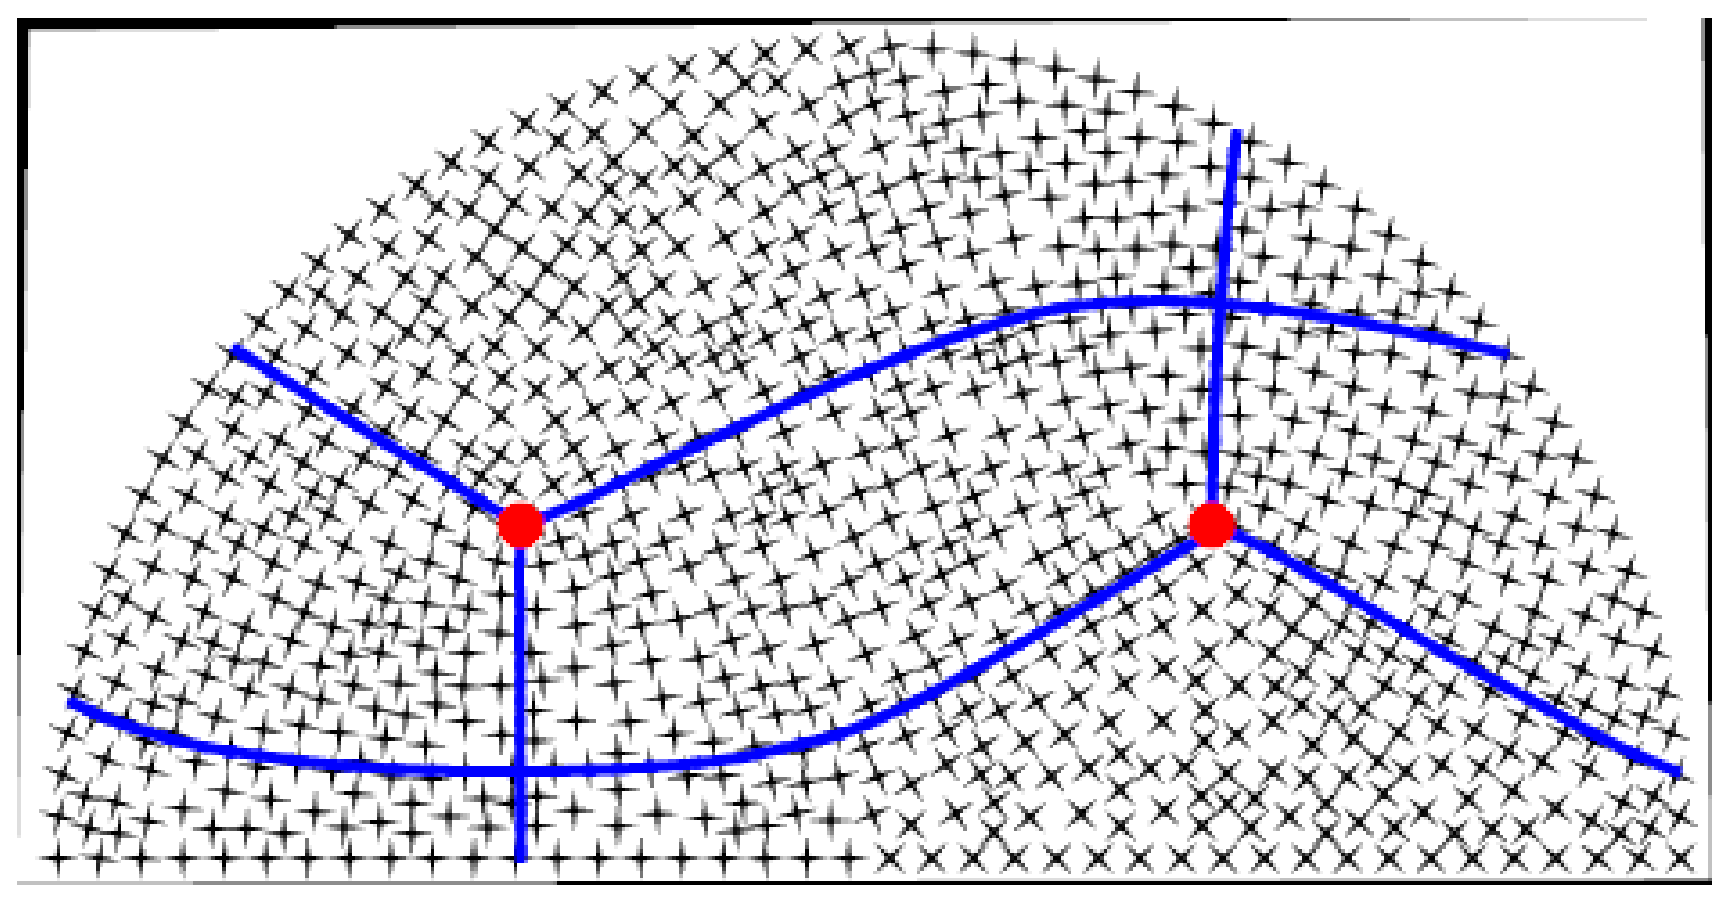
\includegraphics[scale=0.31]{demiDiscValPropNonAligne.eps}
    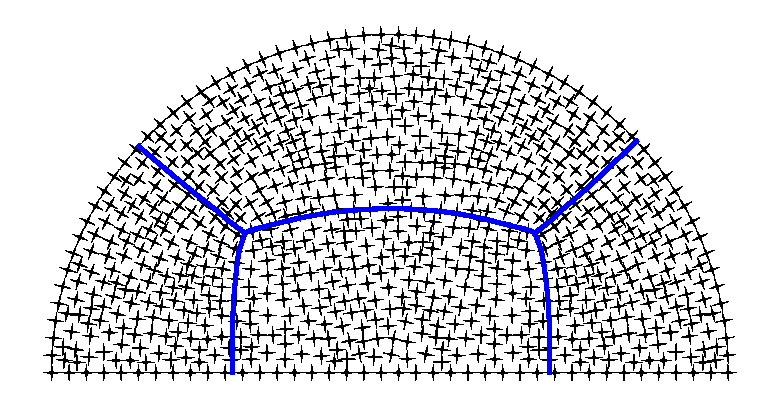
\includegraphics[scale=0.31]{demiDiscValPropAligne.eps}
    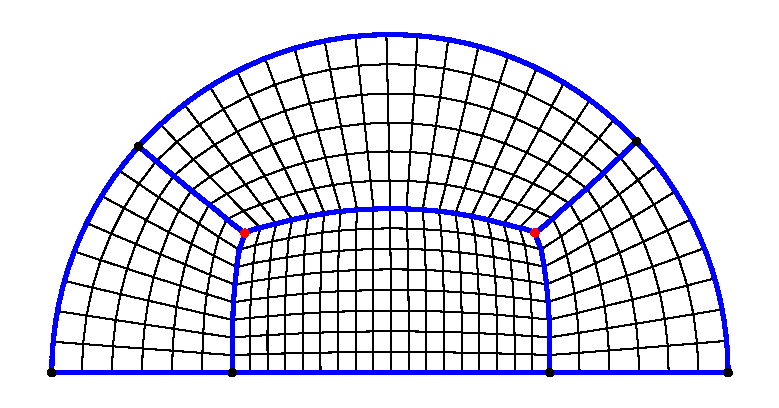
\includegraphics[scale=0.31]{mailDemiDisc.eps}
\end{column}
\begin{column}{0.4\textwidth}
    \centering
    \scriptsize Champ analytique avec 2 zéros\\
    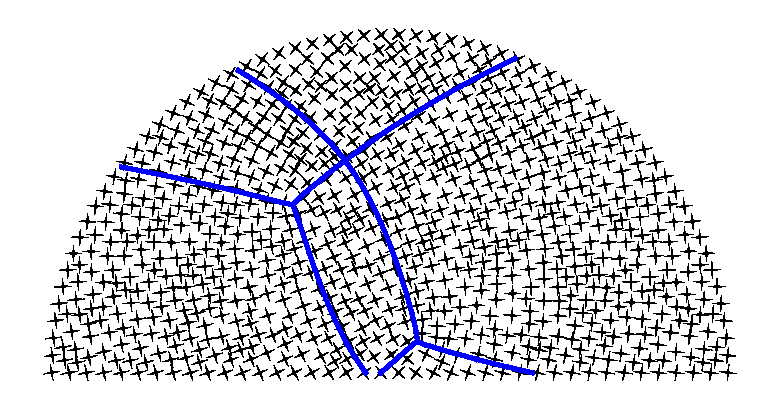
\includegraphics[scale=0.31]{demiDiscGinzNonAligne.eps}
    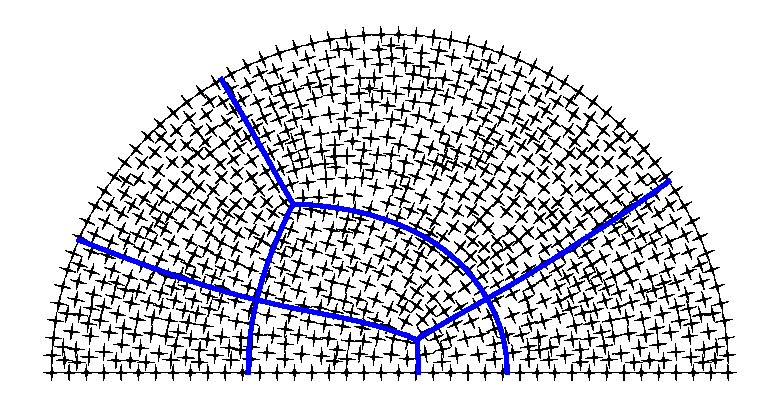
\includegraphics[scale=0.31]{demiDiscGinzAligne.eps}
    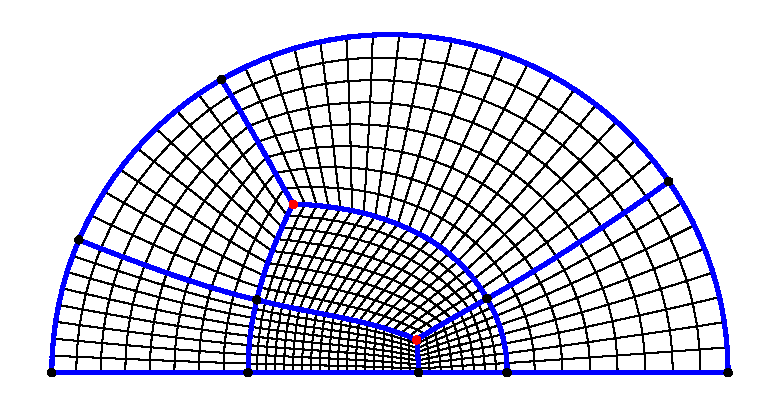
\includegraphics[scale=0.31]{demiDiscMail.eps.eps}
\end{column}
\begin{column}{0.4\textwidth}
    \centering
    \scriptsize Champ analytique avec 3 zéros\\ and 1 point singulier de bord\\
    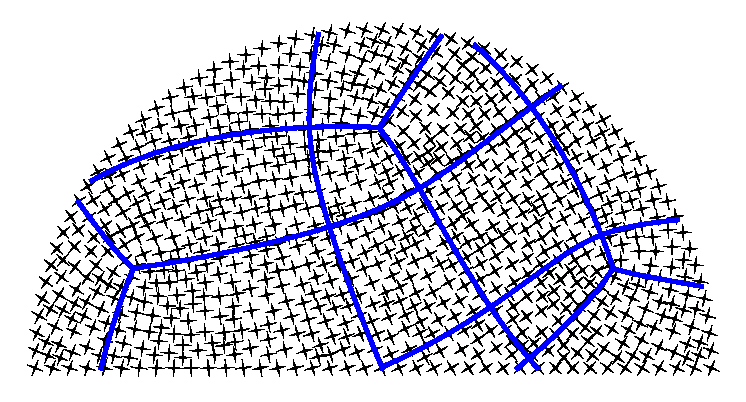
\includegraphics[scale=0.31]{demiDiscTroisPointNonAligne.eps}
    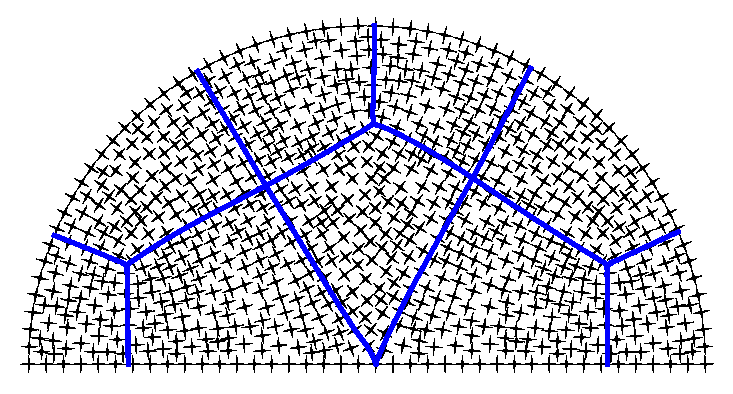
\includegraphics[scale=0.31]{demiDIscTroisPointAligne.eps}
    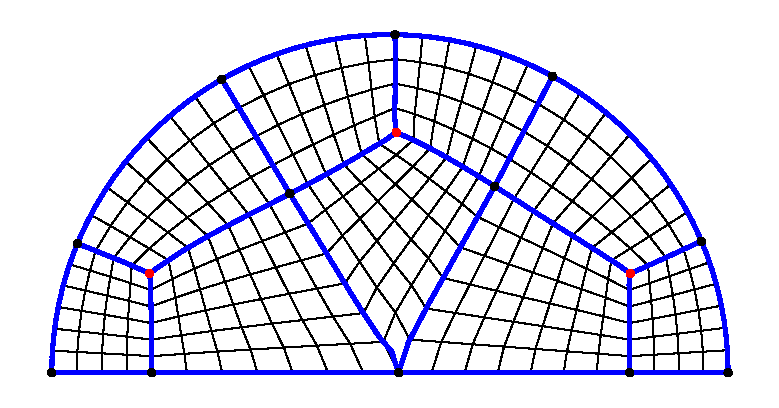
\includegraphics[scale=0.31]{mesh_quad_3.eps}
\end{column}
\end{columns}
\end{frame}

\begin{comment}
\begin{frame}{Domaines non-simplement connexes}{}
\small
\vspace{-0.4cm}
\begin{columns}
\begin{column}{0.65\textwidth}
%\hspace{-0.2cm}
{\bf \color{onera_gray} Domaines à trous, multi-matériaux, ... }\\
\vspace{0.1cm}
\textbf{Application sur un domaine à trou:}\\
\vspace{0.1cm}
Soit $\partial\Omega=\cup_i\Gamma_i$, avec $(b_j^i)_{i,j}$ les points singuliers de bord.\\
\vspace{0.1cm}
La contrainte sur $u$ devient:\vspace{-0.1cm}
\begin{center}
    $deg(u, \partial\Omega)=\sum_i deg(u,\Gamma_i)=\chi(\Omega)-\sum_i\sum_jid(b_j^i).$
\end{center}
\\[-0.1cm]
Ce qui implique $\sum_i(\int_{\Gamma_i}d(\widetilde{\theta_N}-\theta_u))-\sum_i\sum_jid(b_j^i)=0,~~\forall~i$\\
\vspace{0.2cm}
Pour garantir la périodicité de $\phi$ sur chaque $\Gamma_i$, on doit avoir:\vspace{0.02cm}
\begin{center}
    $\int_{\Gamma_i}d(\widetilde{\theta_N}-\theta_u)-\sum_jid(b_j^i)=0,~~\forall~i$
\end{center}
\\[-0.1cm]
Nous construisons un nouveau champ $\widetilde{u}$ à partir de $u$ tel que:\vspace{-0.1cm}
\begin{equation*}
\begin{cases}
   deg(\widetilde{u},\Gamma_0)=1-\sum_j id(b_j^0)\mbox{ sur }\Gamma_0,\\[0.1cm]
   deg(\widetilde{u}, \Gamma_i)=1+\sum_j id(b_j^i),~~~\forall~i.
\end{cases}
\end{equation*}
\end{column}
\begin{column}{0.35\textwidth}
\centering
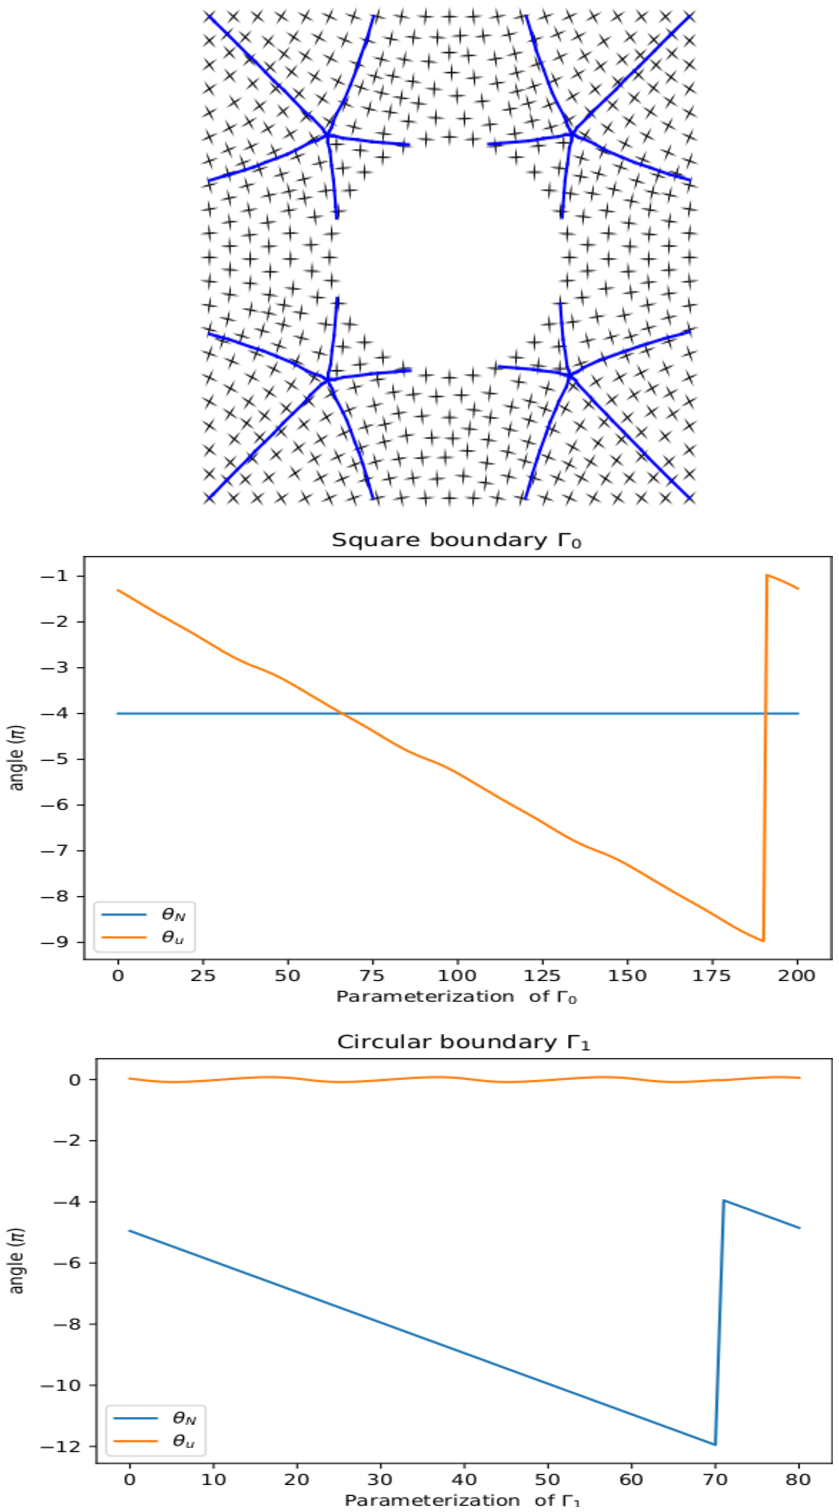
\includegraphics[scale=0.25]{img/courbe_carreDiscVide_english.pdf}
\end{column}
\end{columns}
\end{frame}
\end{comment}

\begin{frame}{Domaines non-simplement connexes}{}
\small
\vspace{-0.3cm}
\begin{columns}
\begin{column}{0.65\textwidth}
%\hspace{-0.2cm}
{\bf \color{onera_gray} Domaines à trous, multi-matériaux, ... }\\
\vspace{0.08cm}
\textbf{Application sur un domaine à trou:}\\
\vspace{0.08cm}
Soit $\partial\Omega=\cup_i\Gamma_i$, avec $(b_j^i)_{i,j}$ les points singuliers de bord.\\
\vspace{0.08cm}
La contrainte sur $u$ devient:\vspace{-0.1cm}
\begin{center}
    $deg(u, \partial\Omega)=\sum_i deg(u,\Gamma_i)=\chi(\Omega)-\sum_i\sum_jid(b_j^i).$
\end{center}
\\[-0.1cm]
Ce qui implique $\sum_i(\int_{\Gamma_i}d(\widetilde{\theta_N}-\theta_u))-\sum_i\sum_jid(b_j^i)=0,~~\forall~i$\\\end{column}
\begin{column}{0.35\textwidth}
\centering
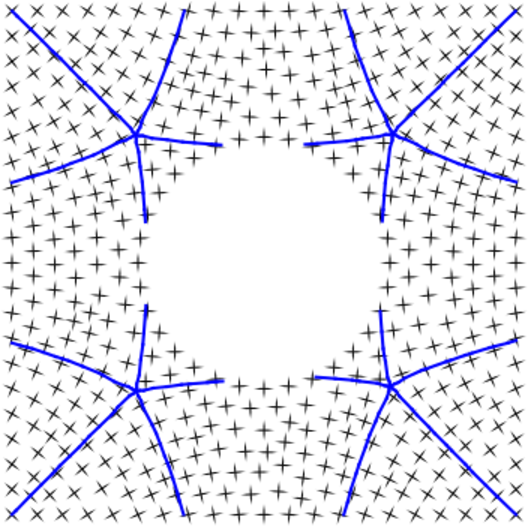
\includegraphics[scale=0.29]{img/carreDiscVide_stream_non_align.pdf}
\end{column}
\end{columns}
\vspace{0.1cm}
\centering
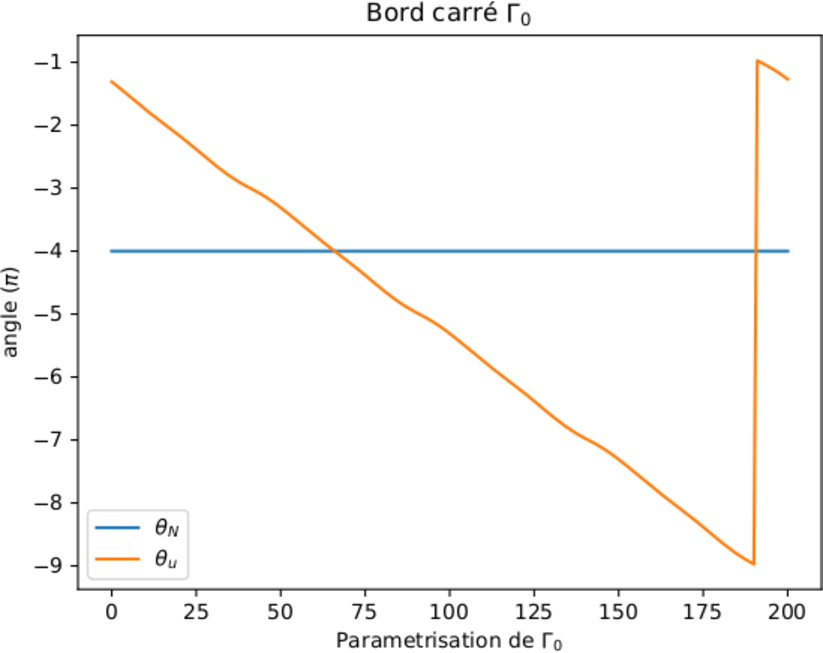
\includegraphics[width=6cm, height=3.1cm]{img/courbe_1.pdf}\hspace{0.6cm}
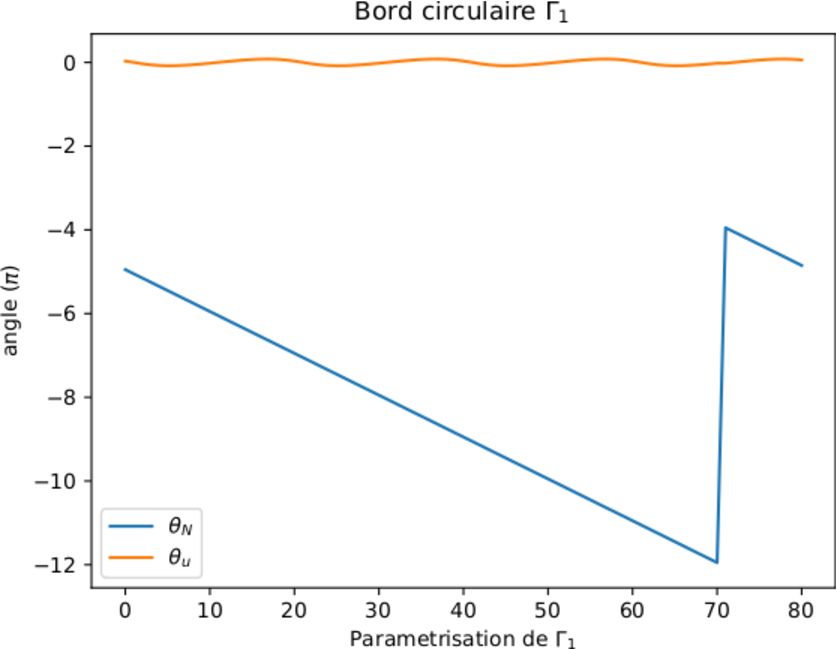
\includegraphics[width=6cm, height=3.1cm]{img/courbe_0.pdf}
\end{frame}

\begin{frame}{Domaines non-simplement connexes}{}
\small
\vspace{-0.4cm}
\begin{columns}
\begin{column}{0.65\textwidth}
%\hspace{-0.2cm}
{\bf \color{onera_gray} Domaines à trous, multi-matériaux, ... }\\
\vspace{0.1cm}
\textbf{Application sur un domaine à trou:}\\
\vspace{0.1cm}
Soit $\partial\Omega=\cup_i\Gamma_i$, avec $(b_j^i)_{i,j}$ les points singuliers de bord.\\
\vspace{0.1cm}
\vspace{0.2cm}
Pour garantir la périodicité de $\phi$ sur chaque $\Gamma_i$, on doit avoir:\vspace{0.02cm}
\begin{center}
    $\int_{\Gamma_i}d(\widetilde{\theta_N}-\theta_u)-\sum_jid(b_j^i)=0,~~\forall~i$
\end{center}
\\[-0.1cm]
Nous construisons un nouveau champ $\widetilde{u}$ à partir de $u$ tel que:\vspace{-0.1cm}
\begin{equation*}
\begin{cases}
   deg(\widetilde{u},\Gamma_0)=1-\sum_j id(b_j^0)\mbox{ sur }\Gamma_0,\\[0.1cm]
   deg(\widetilde{u}, \Gamma_i)=1+\sum_j id(b_j^i),~~~\forall~i.
\end{cases}
\end{equation*}
\end{column}
\begin{column}{0.35\textwidth}
\centering
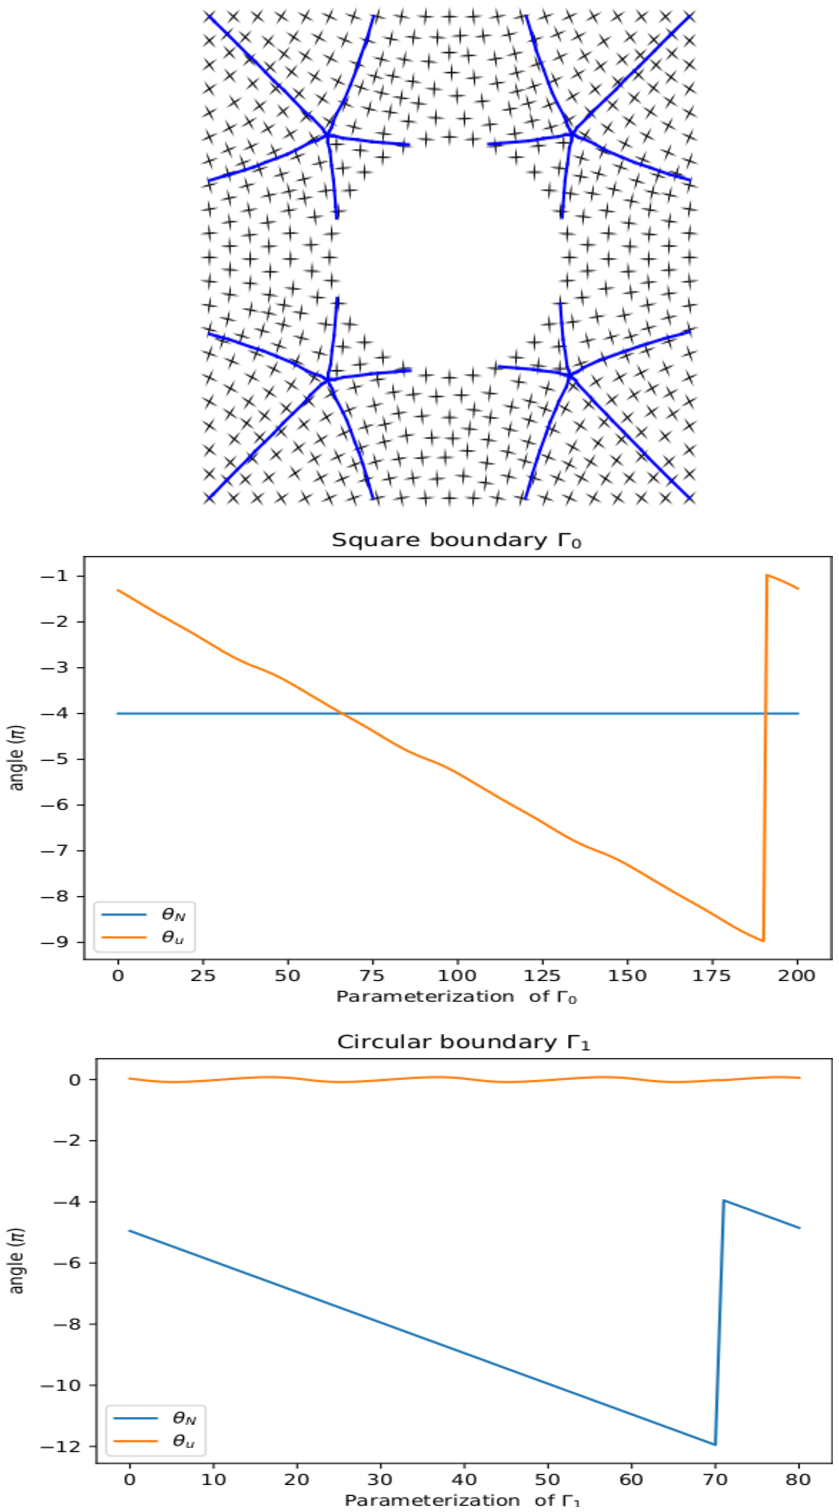
\includegraphics[scale=0.25]{img/courbe_carreDiscVide_english.pdf}
\end{column}
\end{columns}
\end{frame}

\begin{frame}{Domaines non-simplement connexes}
\vspace{-0.35cm}
\begin{columns}
\hspace{-0.25cm}
\begin{column}{0.68\textwidth}
\footnotesize
{\bf Nous introduisons $h:\Omega\longrightarrow\mathbb{R}^2$, %{(\color{onera_gray}constraint field)}
tel que:}
\vspace{-0.15cm}
\begin{equation*}
\begin{cases}
    \triangle h = 0 \mbox{ dans }\Omega,\\
    \displaystyle\frac{1}{2\pi}\int_{\Gamma_0}\theta_h = 4(deg(u, \Gamma_0)-1+\sum_j id(b_j^0))\mbox{ sur } \Gamma_0,\\[0.25cm]
    \displaystyle\frac{1}{2\pi}\int_{\Gamma_i}\theta_h = 4(deg(u, \Gamma_i)-1-\sum_j I(b_j^i)), \forall~i.
\end{cases}
\end{equation*}
\vspace{-0.18cm}
{L'équation du champ d'alignement devient:}
{\color{onera}
\begin{equation*}
\begin{cases}
    \triangle\phi = 0, \mbox{ dans }\Omega\hspace{3.2cm}{\color{red}\rightarrow v=R(\phi)R(\theta_h/4)u}\\
    \phi = \theta_{N_{|\Gamma_i}}-\theta_{u_{|\Gamma_i}}-\frac{1}{4}\theta_{h_{|\Gamma_i}}, \mbox{ sur }\Gamma_i, \forall i
\end{cases}
\end{equation*}
}
\vspace{-0.15cm}
\begin{onerablock}[drop fuzzy shadow]{Théorème 3}
 Soit $u$ un champ de croix tel que $\forall p\in\bar{\Omega}$, ${\bf id(p)<=1/4}$. Etant donné un ensemble $(c_i)_{i\in\{1,\dots,n_b\}}\subset\partial\Omega$ de points distincts tel que la relation (\ref{third_u_c}) est satisfaite, $v=R(\phi)R(\theta_h/4)u$  vérifie le théorème 1 et si aucune de ses séparatrices ne converge en cycle limite.
\end{onerablock}
\end{column}
\begin{column}{0.32\textwidth}
\centering
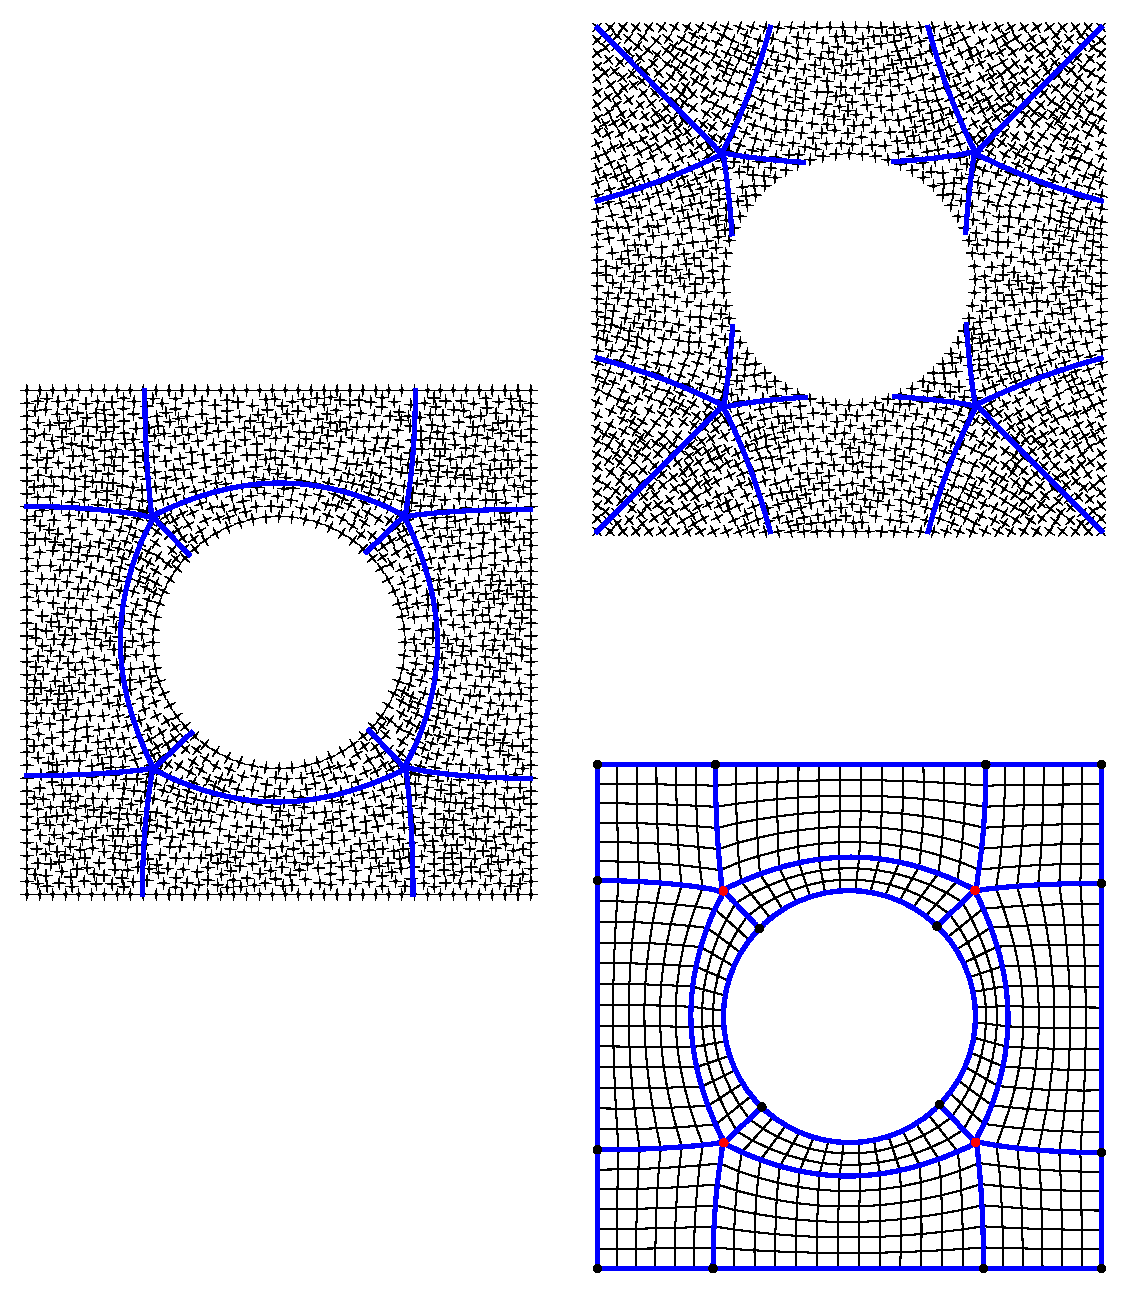
\includegraphics[scale=0.27]{image.eps}
\end{column}
\end{columns}
\end{frame}

\begin{frame}{Exemples}{ Quelques domaines à trous et un domaine avec plusieurs composants connexes}
\vspace{-0.25cm}
\begin{columns}
\begin{column}{0.32\textwidth}
    \centering
    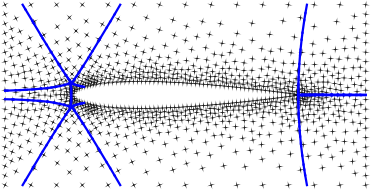
\includegraphics[scale=0.35]{1.png}\vspace{0.6cm}
    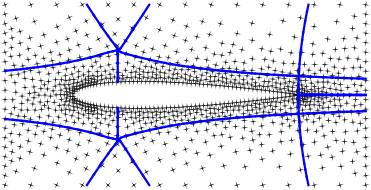
\includegraphics[scale=0.35]{3.png}
\end{column}
\begin{column}{0.32\textwidth}
    \centering
    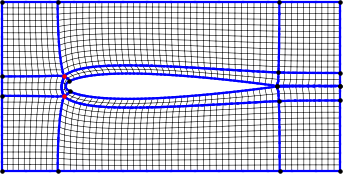
\includegraphics[scale=0.38]{2.png}\vspace{0.6cm}
    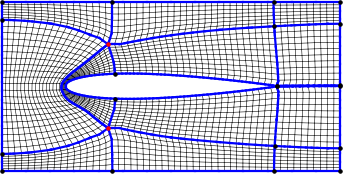
\includegraphics[scale=0.38]{4.png}
\end{column}
\begin{column}{0.32\textwidth}
    \centering
    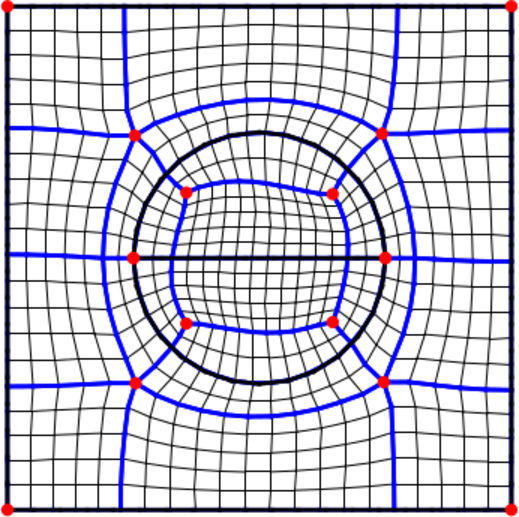
\includegraphics[scale=0.31]{img/mesh_quad_6.pdf}\\\vspace{-0.2cm}
    \scriptsize\color{onera_gray}{ Multi-materiau }
    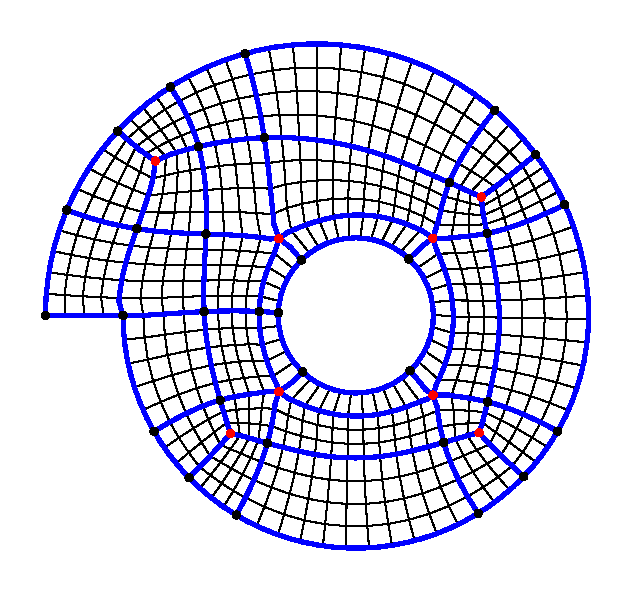
\includegraphics[scale=0.31]{mailNautilus.eps}\\\vspace{-0.1cm}
    \scriptsize\color{onera_gray}{ Nautilus}
\end{column}
\end{columns}
\end{frame}

\begin{frame}{Variétés surfaciques non-planaire}{}
\begin{columns}
\begin{column}{0.45\textwidth}
%\pause[1]
{\bf\color{onera_gray}Gestion de surfaces courbes dans l'espace, surfaces courbes sans bord}\\\vspace{0.2cm}
\begin{itemize}
    \item Formalisme mathématique pensé pour une extension au cadre non-planaire,\\
    \item Les théorèmes 1, 2 et 3 restent valides,\\
    \item Existence de champs vérifiant les contraintes.\\\vspace{0.2cm}
\end{itemize}
%\pause[2]
\textbf{Problème: }{\color{red}Calcul d'angles sur la surface, absence de référence globale}\\
\end{column}
\begin{column}{0.55\textwidth}
%\pause[1]
\centering
\includegraphics[scale=0.65]{img/sphereValPropTrace.png}
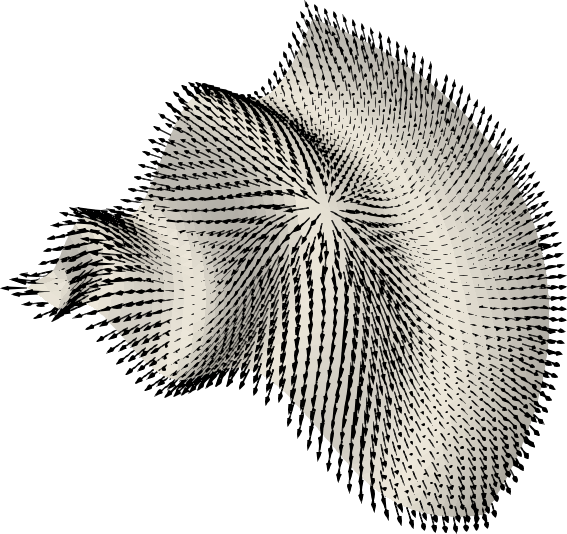
\includegraphics[scale=0.2]{img/vagues_repr.png}\\
\caption{\footnotesize Champ de croix "input"}
\end{column}
\end{columns}
\end{frame}


\begin{frame}{Variétés surfaciques non-planaire}{}
\vspace{-0.5cm}
    {\bf Construction d'une référence globale:}
    \begin{equation*}
        \frac{\partial w}{\partial t} = \nabla^2 w.
        \label{heatequation}
    \end{equation*}
    Propagation d'un vecteur arbitraire en un sommet arbitraire, Conditions de bord de Neumann.\\\vspace{0.2cm}
    \centering
\includegraphics[scale=0.25]{img/vector head method.png}\\
\caption{\footnotesize Vector Heat Method {\color{onera_gray}[K. CRANE et al (2020)]}}
\caption{}
\end{frame}

\begin{frame}{Variétés surfaciques non-planaire}{}
\begin{columns}
\begin{column}{0.5\textwidth}
\begin{itemize}
    %\pause[1]
    \item  Construction d'une référence globale:
    \begin{equation*}
        \frac{\partial w}{\partial t} = \nabla^2 w.
        \label{heatequation}
    \end{equation*}
    Propagation d'un vecteur arbitraire en un sommet arbitraire, Conditions de bord de Neumann.
    %\pause[2]
    \item  Génération d'un champ de croix, tracé des séparatrices, alignement du champ sur le bord, ...
\end{itemize}
\end{column}
\begin{column}{0.5\textwidth}
\centering
%\pause[1]
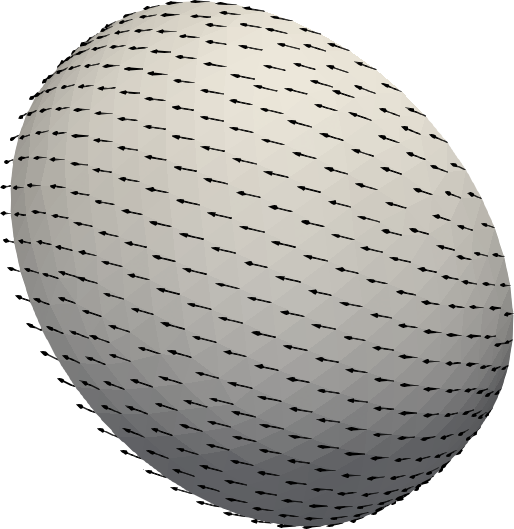
\includegraphics[scale=0.18]{vector.png}
%\pause[2]
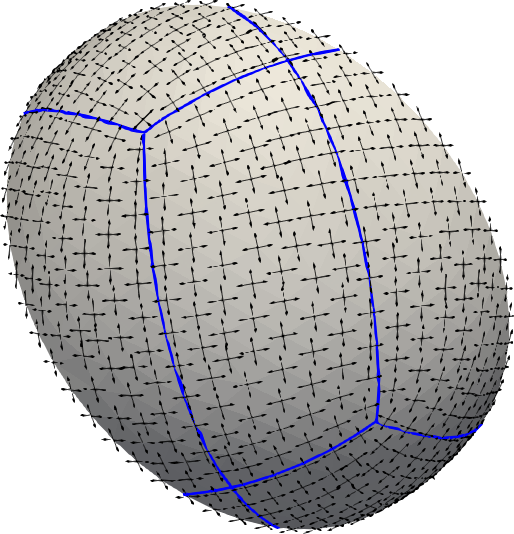
\includegraphics[scale=0.18]{img/nonalign.png}
\end{column}
\end{columns}
\end{frame}

\begin{frame}{Variétés surfaciques non-planaire}
\centering
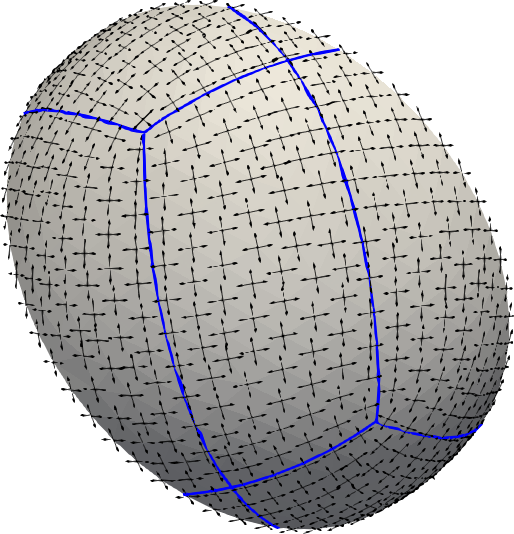
\includegraphics[scale=0.18]{img/nonalign.png}
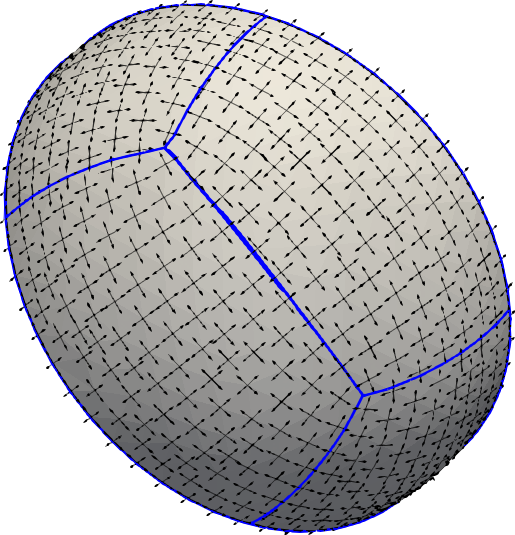
\includegraphics[scale=0.18]{img/align.png}
\includegraphics[scale=0.18]{img/quart_quad_1.png}
\includegraphics[scale=0.178]{img/quart_quad_2.png}
\end{frame}


\begin{frame}{Conclusion et perspectives}
\begin{columns}
    \begin{column}{0.6\textwidth}
    \only<1>{
    {\color{onera}Conclusion:}\\\vspace{0.15cm}
    \begin{itemize}
        \item Mise en place d'un cadre permettant la génération d'un "mesh quad" à partir de champs de croix "arbitraires",\\\vspace{0.15cm}
        \item Homogénéité, points singuliers de bord, domaines non simplement connexes, variétés surfaciques non-planaires {\color{onera_gray}(sans projection sur le plan, natif de la surface)}, ...\\\vspace{0.15cm}
        \item Implémentation d'un code C++/Python %{\bf (HQMesh)} réalisant les résultats.
    \end{itemize}
    }
    \only<2>{
    {\color{onera}Perspectives:}\\\vspace{0.15cm}
    \begin{itemize}
        %\item Surfaces courbes dans l'espace\vspace{0.1cm}
        \item Automatisation de la génération du champ de croix "input" par rapport à des propriétés données {\color{onera_gray} (homogénéité, numérotation de noeuds, ... )}\\\vspace{0.15cm}
        \item Adaptation de maillage à partir de cartes d'erreur à postériori,\\\vspace{0.15cm}
        %\item Optimisation du code HQMesh,\\\vspace{0.15cm}
        \item Extension de la méthode à des domaines volumiques\vspace{0.15cm}
    \end{itemize}
    }
    \end{column}
    \begin{column}{0.4\textwidth}
        \centering
        \includegraphics[scale=0.3]{img/vagues.png}
    \end{column}
\end{columns}
\end{frame}


